\documentclass[12pt]{article}

% Set up data, if you need to add a package, go here
%Adapted from Adapted from UWA Engineering Final Year Project.


%\usepackage[utf8]{inputenc}
\usepackage[x11names,dvipsnames,svgnames,table]{xcolor}

% general incantations
\usepackage[export]{adjustbox}
\usepackage{afterpage}

\usepackage{graphicx}
\usepackage{placeins}
\usepackage{pdfpages}
\usepackage{algorithm2e}
\usepackage{array}
\usepackage{booktabs}
\usepackage[most]{tcolorbox}
\usepackage{calligra}
\usepackage{caption}
\usepackage{datetime}
%\usepackage{dblfnote}
\usepackage{dirtytalk}
\usepackage{dsfont}
\usepackage{etex}
\usepackage{fancyhdr}
\usepackage{fix-cm}
\usepackage[T1]{fontenc}
\usepackage{textcomp,gensymb} %for \degree C symbol
\usepackage{graphicx}
\usepackage{lipsum}
\usepackage{listings}
\usepackage{transparent}
\usepackage[everyline=true,framemethod=tikz]{mdframed}
\usepackage{mparhack}
\usepackage{multicol}
\usepackage{multirow}
\usepackage{parskip}
\usepackage{lscape}
\usepackage{pdflscape}
\usepackage{pdfpages}
\usepackage{placeins}
\usepackage[document]{ragged2e}
\usepackage{rotating}
\usepackage{setspace}
\usepackage{subcaption}
\usepackage{threeparttable}
\usepackage[normalem]{ulem}
\usepackage{verbatim}
\usepackage{soul} %highlighting, strike through etc.

%Automated appendices
\usepackage[titletoc,title,header]{appendix} %advanced functionality

%language settings
\usepackage[utf8]{inputenc}
\usepackage[australian]{babel}
\usepackage{csquotes}

%page setup
%this where we adjust the binding offset, if relevant
\usepackage[a4paper]{geometry}
\usepackage{lastpage} % for page 1 of n footers

%cross referencing
\usepackage{hyperref}

%maths stuff
\usepackage{amsmath}
\usepackage{mathtools}

\setcounter{secnumdepth}{5}

%lists
\usepackage{enumitem}

%working collaboratively
\usepackage[backgroundcolor=yellow]{todonotes}

% bibliography file using harvard
\usepackage[round, sort, numbers, authoryear]{natbib}

%glossary for acronyms
\usepackage[acronym,nonumberlist,toc,section=subsection,numberedsection=nolabel]{glossaries} 
\makeglossaries

%line spacing
\linespread{1.25}


\begin{document}

\thispagestyle{empty}
\setlength\headheight{0pt} 
\begin{center}

\begin{center}

\includegraphics[width=0.65\linewidth]{images/UL_logo.jpg}            
\end{center}	

        \vspace{0.25cm}
        {\scshape\LARGE University of Limerick \par}
        \vspace{0.25cm}
        {\scshape\Large CS4157 Software Quality\par}
        \vspace{0.5cm}

        {\Large\bfseries The Role \& Importance of Testing in Facilitating the Development of Quality Software\par}
        
        \vspace{0.5cm}
        {\Large\itshape Niall Dillane\par}
        CSIS
        \vspace{0.25cm}

\vspace{1cm}
Submitted to\par
Dr. Valentine Casey \\
CSIS\par
\vspace{1.5cm}
\large
\today

\end{center}

\clearpage
\restoregeometry
\justify

\section*{Abstract}
Present thesis abstract here, typically there are no references, figures or tables in the abstract.
\pagebreak


\tableofcontents
\pagebreak


\section{Introduction}
\subsection{Subsection Example}
I am a subsection
\subsubsection{Sub Subsection Example}
I am a sub subsection
\pagebreak

\begin{itemize}
    \item{Research and discuss the role and importance of dynamic analysis in the verification and validation of software and the essential part it plays in facilitating quality.}
    \item{Clearly outline and define what Functional and Non-Functional Software Requirements are and in your discussion compare and contrast the differences between them.}
    \item{Outline and discuss the key stages in the software testing process}
    \item{Research and define the principles of an effective test strategy.}
    \item{Research and discuss how Functional Software Requirements and Non- Functional requirements can be successfully tested and define the differences in approach required by each.}
    \item{Define and discuss the importance of utilizing both white box and black box testing.}
    \item{Consider and discuss the role and importance of having documented test procedures in place to facilitate effective testing.}
    \item{Research and outline the purpose, importance and content of a test plan}
    \item{Consider each of the following and outline and describe their role and
    purpose in the testing process:}
        \begin{itemize}
        \item{Unit Testing}
        \item{Integration Testing}
        \item{Regression Testing}
        \item{System Testing}
        \item{Acceptance Testing}
        \end{itemize}
\end{itemize}


\pagebreak
\section{Sample Table}
\begin{table}[ht!]
\centering
    
	\caption{Comparison \textit{p} values}
	\begin{tabular}{ |l|c|c|}	
		\hline		
		\textbf{Attribute} & \textbf{\textit{p-value}} & \textbf{Significant} \\ \hline
		Model A	 & 0.0521 & N \\ \hline
		Model B  & 0.6171 & N \\ \hline 
		Model C  & <0.00001 & Y \\ \hline 
	\end{tabular}
	\label{tab:pvalues}
\end{table} 


\subsubsection{Sample Figure}
\begin{figure}[ht!]
 	\centering
 	\caption{Perceptron (Artificial Neural Network)}
 	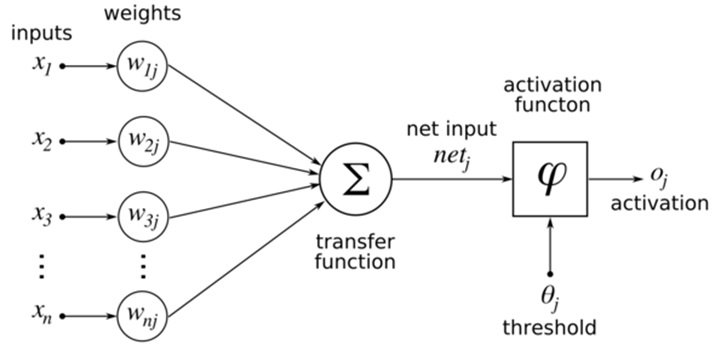
\includegraphics[width=0.7\linewidth]{images/ANN.jpg}
 	\label{lab:perceptron}
 \end{figure}
\pagebreak




%prints bibliography from bibliography file.
\bibliographystyle{agsm}
\renewcommand{\bibname}{References} % changes the header; default: Bibliography
\bibliography{bibliography.bib} % with extension

\end{document}
